\section{Packaging \& Deployment}

% --- SLIDE 1: WHAT IS THE MODEL ---
\begin{frame}{``Ship the Model'' --- Ship \emph{What}, Exactly?}

    \centering
    \resizebox{0.98\textwidth}{!}{%
    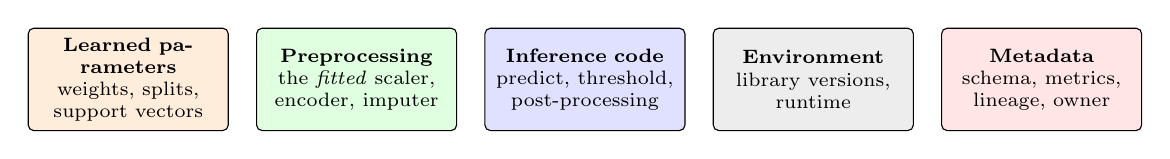
\begin{tikzpicture}[
        b/.style={rectangle, draw, rounded corners=2pt, minimum height=1.3cm, text width=2.4cm,
                  align=center, font=\scriptsize, inner sep=2pt}
    ]
        \node[b, fill=orange!14] (w)   at (0,0)    {\textbf{Learned parameters}\\weights, splits, support vectors};
        \node[b, fill=green!12]  (pre) at (2.9,0)  {\textbf{Preprocessing}\\the \emph{fitted} scaler, encoder, imputer};
        \node[b, fill=blue!12]   (code)at (5.8,0)  {\textbf{Inference code}\\predict, threshold, post-processing};
        \node[b, fill=gray!14]   (env) at (8.7,0)  {\textbf{Environment}\\library versions,\\runtime};
        \node[b, fill=red!10]    (meta)at (11.6,0) {\textbf{Metadata}\\schema, metrics, lineage, owner};
    \end{tikzpicture}}

    \vspace{1.0em}
    \begin{itemize}
        \item Forgetting the \textbf{fitted} preprocessing is the classic production bug: a scaler refitted
              on the serving batch silently rescales everything and the model quietly degrades.
        \item Forgetting the \textbf{input schema} means you discover a renamed column at 3am rather than
              at deploy time.
        \item Forgetting the \textbf{owner} means nobody is paged when it breaks.
    \end{itemize}

    \vspace{0.6em}
    \begin{block}{Rule}
        Serialise the \textbf{whole pipeline} --- \texttt{Pipeline([("scale", ...), ("clf", ...)])} --- never
        the estimator alone. One artifact, one \texttt{predict}, no room for skew.
    \end{block}

\end{frame}
